\documentclass{article}
\usepackage[a4paper, total={6in, 8in}]{geometry}
\usepackage[utf8]{inputenc}
\usepackage{amsmath}
\usepackage{amssymb}
\usepackage{xcolor}
\usepackage{tabularx}
\usepackage{booktabs}
\usepackage{multirow}
\usepackage{graphicx}
\graphicspath{ {./imgs/} }
\usepackage{biblatex}
\addbibresource{liography.bib}
\usepackage{amsthm}
\usepackage{float}

\newtheorem{theorem}{Theorem}[section]
\newtheorem{corollary}{Corollary}[theorem]
\newtheorem{lemma}[theorem]{Lemma}
\newtheorem{definition}{Definition}[section]
\newtheorem{assumption}{Assumption}[section]

\DeclareMathOperator*{\argmax}{argmax}
\DeclareMathOperator*{\argmin}{argmin}

\title{Quantized Q-Learning for Near-Optimal Quantizers}
\date{\today}
\author{Liam Cregg}

\begin{document}

\begin{titlepage}
    \maketitle
\end{titlepage}

\newpage

% Intro to zero-delay quantizers, summarize results from "Zero-Delay Lossy Coding"
\section{Zero-Delay Lossy Coding and Optimal Quantizers}\label{optimal quantizers}
We are interested in a variant of Shannon's lossy source coding problem: Given an information source \( \{X_t\}_{t\ge0} \) from a finite alphabet \( \mathbb{X} \), we wish to compress this source at rate \(R\) bits per source symbol, and then reproduce the source as \( \{\hat{X}_t\}_{t\ge0} \), where \(\hat{\mathbb{X}}\) is the (also finite) reproduction alphabet. In particular, a \((2^{RT},T)\) block code encodes T source symbols \(X_{[0,T-1]}\) as \(\eta^T : \mathbb{X}^T \to \{1,\ldots,2^{RT}\} \), and decodes them as \( \gamma^T : \{1,\ldots,2^{RT}\} \to \hat{\mathbb{X}}^T \). The goal is often to minimize the distortion, given by %chktex 3

\[ D_T(R) := \frac{1}{T} E[\sum_{t=0}^{T-1}d(X_t,\hat{X_t})]\] %chktex 3

We call a rate-distortion pair \((R,D)\) achievable if there exists a sequence of \((2^{RT},T)\) codes \((\eta^T,\gamma^T)\) such that

\[ \limsup_{T \to \infty}D_T(R) \le D\]

The minimum achievable distortion for a given rate \(R\) is denoted by \(D(R)\), and classically we can obtain this distortion by taking the block length \(T\) to infinity (provided that the source is stationary and ergodic), i.e.

\[D(R) = \lim_{T \to  \infty}D_T(R)\]

However, this approach requires encoding very large blocks of data at a time, and hence incurs large delay. This delay may not be allowable in many real-time applications, and so we tackle a variant of this lossy coding problem, where we enforce zero delay (hence a block coding approach is not viable). We will assume throughout that the source \( \{X_t\}_{t \ge 0} \) is a discrete-time Markov process with probability matrix \( P \), which is irreducible and aperiodic (and thus admits a unique invariant measure, denoted by \( \pi_0 \)). After encoding, the (compressed) information is sent over a discrete noiseless channel with input and output alphabets \( \mathcal{M} := \{1,\ldots,M\} \). %chktex 3

Thus, the encoder is defined by a quantization policy \( \Pi = \{\eta_t\}_{t \ge 0} \), where \( \eta_t : \mathcal{M}^t \times \mathbb{X}^{t+1} \to \mathcal{M} \). That is, the encoder can use all past quantization outputs and all past and current source inputs to generate the current quantization output. This can be viewed as the quantization policy selecting a quantizer \( Q_t : \mathbb{X} \to \mathcal{M} \) using past information, then quantizing \( X_t \) as \( q_t = Q_t(X_t) \)~\cite{Linder}. Then, the decoder generates the reconstruction \( \hat{X}_t \) without delay, using decoder policy \( \gamma = \{\gamma_t\}_{t \ge 0} \), where \( \gamma_t : \mathcal{M}^{t+1} \to \hat{\mathbb{X}} \). Thus we have \( \hat{X}_t = \gamma_t(q_{[0,t]}) \). Note that, since the source alphabet is finite, there exists an optimal decoding policy for every encoding policy. Thus, we restrict our search to finding an optimal encoding policy and assume the corresponding optimal decoding policy is used. %chktex 3

In general, for the zero-delay coding problem, the goal is to minimize the average cost/distortion. In the infinite horizon case with cost function/distortion measure \( c : \mathbb{X} \times \hat{\mathbb{X}} \to [0,\infty) \), this is given by: %chktex 9
\[ J(\pi_0, \Pi, \gamma) := \limsup_{T\to\infty}\mathbf{E}_{\pi_0}^{\Pi, \gamma}\left[\frac{1}{T}\sum_{t=0}^{T-1}c(X_t,U_t)\right] \]

However, for the time being we will consider the discounted cost problem, as this problem is easier to tackle using Q-learning methods (to be discussed later). Thus, for some \( \beta \in (0,1) \), we wish to minimize:
\[ J_{\beta}(\pi_0, \Pi, \gamma) := \lim_{T\to\infty}\mathbf{E}_{\pi_0}^{\Pi, \gamma}\left[\frac{1}{T}\sum_{t=0}^{T-1}\beta^t c(X_t,U_t)\right] \]

For the finite horizon problem, policies using only the conditional probability measure \( \pi_t = P(x_{t+1}|q_{[0,t-1]}) \) and \( x_t \) to generate \( q_t \) have been shown to be optimal by Walrand and Varaiya~\cite{Walrand}. That is, for every admissable policy, there exists a policy of the form \( Q_t = \eta_t(\pi_t) \) and \( q_t = Q_t(X_t) \) that performs at least as well. Such policies are called Walrand-Varaiya type or Markov policies, and denoted by \( \Pi_{W} \). If \( \eta_t \) does not depend on \( t \), we call such policies stationary and denote the set of these policies by \( \Pi_{WS} \). In~\cite{Wood}, Walrand and Varaiya's result was also shown to apply to the infinite horizon discounted cost problem, and in fact that the optimal policy is stationary (that is, there exists an optimal (deterministic) quantization policy in \( \Pi_{WS} \) for the infinite horizon discounted cost problem).

Importantly, it was shown in~\cite{Wood} that \( \pi_{t+1} \) is conditionally independent of \( (\pi_{[0,t-1]}, Q_{[0,t-1]}) \) given \( \pi_t \) and \( Q_t \), and hence \( \{\pi_t\} \) is a controlled Markov process with control \( \{Q_t\} \). Using conditional probability properties, we obtain the update equation for \( \pi_t \):

\begin{equation}
    \pi_{t+1}(x_{t+1}) = \frac{1}{\pi_t(Q^{-1}(q_t))}\sum_{x_t \in Q^{-1}(q_t)}P(x_{t+1}|x_t)\pi_t(x_t)\label{eq:1}
\end{equation}

% Motivation: value iterations etc. is very difficult (not just computationally but also algorithm design, given the setup of problem)
Therefore, in theory one could use dynamic programming principles to run an iteration algorithm on this controlled Markov process in order to obtain the optimal policy \( \Pi \in \Pi_{WS} \). However, in practice this proves to be difficult (see e.g.~\cite{Wood}), and hence we propose to use Q-learning in order to find the optimal quantization policy. To this end, we will utilize the recent work of~\cite{Kara} in the near-optimality of policies obtained through Q-learning under quantization. First, we will need some results on the properties of the controlled Markov process \( \{\pi_t\} \).

\subsection{A Topology on Quantizers}
As we will be discussing convergence and continuity regarding quantizers, we need to define an appropriate topology. Viewing a quantizer \( Q \) as a map from \( \mathbb{X} \) to \( \mathcal{M} \), we denote the \( i^{th} \) \emph{bin} of \( Q \) as \( B_i = Q^{-1}(i), i=1,\ldots,M \), and we denote the set of all possible quantizers by \( \mathcal{Q} \). Following~\cite{Linder}, we note that a quantizer with bins \( \{B_1,\ldots,B_M\} \) can alternatively be represented as a stochastic kernel from \( \mathbb{X} \) to \( M \) such that \( Q(i|x) = 1_{x \in B_i}, i=1,\ldots,M \). Then if \( P \) is a probability measure on \( \mathbb{X} \), we denote by \( PQ \) the joint probability measure \( PQ(x,y) = P(x)Q(y|x) \). If we introduce the equivalence relation \( Q \equiv Q' \) iff \( PQ = PQ' \), then we can imbue these equivalence classes with the weak convergence topology (that is, we say \( Q_n \to Q \) iff \( PQ_n \to PQ \)). Under this topology,~\cite{Linder} showed the following lemma for the controlled Markov chain \( \{\pi_t\} \).

\begin{lemma}\label{lemma:weak}~\cite[Lemma 11]{Linder}.
    The transition kernel \( P(d\pi_{t+1}|\pi_t,Q_t) \) is weakly continuous in \( (\pi_t,Q_t) \). That is,

    \[ \int_{\mathcal{P}(\mathbb{X}) \times \mathcal{Q}} f(\pi^{'})P(d \pi^{'}|\pi, Q) \]

    is continuous on \( \mathcal{P}(\mathbb{X}) \times \mathcal{Q} \) for all continuous and bounded \(f\).
\end{lemma}

\begin{proof}
    The proof can be found in its entirety in~\cite{Linder}, but essentially follows by writing the integral as a sum over \( \mathcal{M} \), and using the additional fact that \( \pi_n Q_n \to \pi Q \) in total variation.
\end{proof}

\section{Unique Ergodicity of \( \{\pi_t\} \)}\label{section:unique-ergodicity}
A desirable feature of \( \{\pi_t\} \) (and one that we will need later for Q-learning) is that under a random exploration policy \( \Pi^* \), the process admits a unique invariant measure. To prove this, note that under a randomized policy, we can view a given quantizer output \( q_t \) as an observation \( Y_t \) (living in \( \mathbb{Y} := \mathcal{M} \)) of the true state \( X_t \), dependent on an i.i.d noise variable \( Z_t \). More concretely, let \( m := |\mathcal{Q}| \) (\( m \) is finite since \( \mathbb{X} \) is finite). Then enumerate the quantizers in \( \mathcal{Q} \) from 1 to \( m \), i.e. \( \mathcal{Q} = \{ Q_1,\ldots,Q_m \} \). Finally, let \( y_t := q_t = h(x_t,z_t) = Q_{z_t}(x_t) \), where \( Z_t \) is an i.i.d random variable taking values in \( \mathcal{Z} := \{1,\ldots,m\} \). Then we can use some tools from the literature of Partially Observed Markov Processes (POMPs) to determing the ergodicity of \( \{\pi_t\} \).

\subsection{Predictor and Filter Merging}

For a fixed \( x \in \mathbb{X} \), we denote \( h(x,\cdot) := h_x(\cdot) : \mathcal{Z} \to \mathbb{Y} \), and let the noise process \( \{Z_t\}_{t\ge0} \) have probability measure \( Z_0 \sim R \). Since the noise process is assumed independent of the state process \( \{X_t\}_{t\ge0} \), we can write the following update equation for the joint process \( \{X_t,Y_t\}_{t\ge0} \) %chktex 3

\[ P((X_{t+1},Y_{t+1}) | (X,Y)_{[0,t]} = (x,y)_{[0,t]}) = R(h_{x+1}^{-1}(y_{t+1}))P(x_{t+1} | x_t) \] %chktex 3

It follows that \( \{X_t,Y_t\}_{t\ge0} \) is Markov, with a probability measure on \( \mathbb{X}^{\mathbb{Z}_{\ge0}} \times \mathbb{Y}^{\mathbb{Z}_{\ge0}} \), endowed with the product topology. Since this measure depends on the distribution of \( X_0 \), we denote this measure by \( P^\mu \) where \( X_0 \sim \mu \). %chktex 3

Given the above characterization, we can view \( \pi_t \) as what is known as a \emph{predictor} in the POMDP literature (that is, \( \pi_t(x_t) = P(x_t | y_{[0,t-1]}) \)). Recall the recursion equation~\eqref{eq:1} and note that this is dependent on the initialization of \( \pi_0 \), also called the \emph{prior}. We denote the predictor process resulting from the prior \( \nu \) as \( \{\pi_t^\nu \}_{t\ge0} \). A common question in the POMDP literature is when measures such as the predictor are \emph{stable}, which essentially means that the process eventually forgets an incorrect prior, i.e. \( \nu \neq \mu \). More formally, we introduce the following definitions %chktex 3

\begin{definition}\label{definition:weak_merge}
    Two sequences of probability measures \( \{P_t\}_{t\ge0} \) and \( \{Q_t\}_{t\ge0} \) merge weakly if \( \forall f \in C_b(\mathbb{X}) \), we have \( \lim_{t \to \infty} |\int fdP_t - \int fdQ_t| = 0\). %chktex 3 chktex 21
\end{definition}

\begin{definition}\label{definition:TV_merge}
    For two probability measures \( P \) and \( Q \), the total variation norm is given by \( ||P-Q||_{TV} = \sup_{||f||_\infty \le 1} |\int fdP - \int fdQ| \) for f measurable.
\end{definition}

\begin{definition}\label{definition:weak_stable}
    A predictor process is stable in the sense of weak merging in expectation if for any \( f \in C_b(\mathbb{X}) \) and any prior \( \nu \) with \( \mu \ll \nu \), we have \( \lim_{n \to \infty}E^\mu [|\int fd\pi_t^\mu - \int fd\pi_t^\nu|] = 0 \). %chktex 3
\end{definition}

\begin{definition}\label{definition:TV_stable}
    A predictor process is stable in the sense of total variation in expectation if for any prior \( \nu \) with \( \mu \ll \nu \), we have \( \lim_{n \to \infty}E^\mu [||\pi_t^\mu - \pi_t^\nu||_{TV}] = 0 \). %chktex 3
\end{definition}

Note that merging (respectively, stability) in total variation implies merging (respectively, stability) weakly since \( C_b(\mathbb{X}) \) is a subset of measurable and bounded functions.

The above definitions are of interest due to a result from~\cite[Theorem 2]{Stettner} relating stability to ergodicity. We state and prove a slightly modified version of this result here, adapted for our setup.

\begin{theorem}\label{theorem:unique}
    Assume that there exists a unique invariant measure \( \zeta(dx,dy) \) for the Markov process \( \{X_t,Y_t\}_{t\ge0} \) and that the predictor process \( \{\pi_t^\mu \}_{t\ge0} \) is stable in the sense of~\ref{definition:weak_stable}. Then there is at most one invariant measure for the the joint Markov process \( \{X_t,Y_t,\pi_t^\nu \} \) for any prior \( \nu \). %chktex 3
\end{theorem}

\begin{proof}
    Assume that \( m_1,m_2 \in \mathcal{P}(\mathbb{X} \times \mathbb{Y} \times \mathcal{P}(\mathbb{X})) \) are two invariant measures for the joint process \( \{X_t,Y_t,\pi_t^\nu \} \). Then their projections on \( \mathbb{X} \times \mathbb{Y} \) are invariant for \( \{X_t, Y_t\}_{t\ge0} \). Then, by unique invariance of \( \zeta(dx,dy) \) we have %chktex 3
    \[ m_i(dx,dy,d\nu) = P_{m_i}(d\nu | x,y)\zeta(dx,dy) \]

    Then we show that \( m_1(F) = m_2(F) \) for each \( F \) on a set of measure-determining functions~\cite{Stettner}, namely those s.t. \( F(x,y,\nu) = \phi(x,y)H(\nu(\phi_1),\ldots,\nu(\phi_l)) \), where \( \phi \in C(\mathbb{X} \times \mathbb{Y}), \phi_1,\ldots,\phi_l \in C(\mathbb{X}), H \) is bounded and Lipschitz continuous with constant \( L_H \), and \( l \in \mathbb{N} \).

    Let \( S \) be the transition operator associated with the process \( \{X_t,Y_t,\pi_t^\nu \} \). Then by invariance we have for \( i=1,2 \)

    \[ m_i(F) =  \int_{\mathbb{X} \times \mathbb{Y} \times \mathcal{P}(\mathbb{X})} \frac{1}{n}\sum_{j=0}^{n-1}S^j F(x,y,\nu)P_{m_i}(d\nu | x,y)\zeta(dx,dy) \]

    And thus,
    \begin{align*}
            & |m_1(F) - m_2(F)|                                                                                                                                                                                                                                             \\
        \le & \int_{\mathbb{X} \times \mathbb{Y} \times \mathcal{P}(\mathbb{X}) \times \mathcal{P}(\mathbb{X})} \frac{1}{n}\sum_{j=0}^{n-1} |S^j F(x,y,\nu_1) - S^j F(x,y,\nu_2)|P_{m_1}(x,y,\nu_1)P_{m_2}(x,y,v_2)\zeta(dx,dy)                                             \\
        \le & L_H ||\phi|| \int_{\mathbb{X} \times \mathbb{Y} \times \mathcal{P}(\mathbb{X}) \times \mathcal{P}(\mathbb{X})} \frac{1}{n}\sum_{j=0}^{n-1}E_{xy}[\sum_{i=1}^{l}|\pi_j^{\nu_1}(\phi_i) - \pi_j^{\nu_2}(\phi_i)|]P_{m_1}(x,y,\nu_1)P_{m_2}(x,y,v_2)\zeta(dx,dy)
    \end{align*}
    Since the predictors are stable in the sense of~\ref{definition:weak_stable}, and by the dominated convergence theorem, the last line converges to zero as \( n \to \infty \).
\end{proof}

It can be shown through a tightness argument (see~\cite[Theorem 3]{Stettner}) that the above also implies that the Markov process \( \{Y_t,\pi_t^\nu \} \) has at most one invariant measure.

\subsection{Predictor Stability}
In light of~\ref{theorem:unique}, we want to show that our predictor process \( \{\pi_t\}_{t\ge0} \) is stable in the sense of~\ref{definition:weak_stable}. While stability (and even unique ergodicity) of the predictor have been studied extensively (see e.g. \cite{Chigansky}, \cite{DM} for discussions), the assumptions of these theorems are in general quite strong, and usually not applicable for large classes of sources. For example, they may require that the state has a uniformly positive transition density, etc.~\cite{Chigansky}. %chktex 3 %chktex 2

In order to generalize our sources and quantizers as much as possible, we will utilize results in~\cite{Curtis}, which relate the stability of the predictor to stability of the \emph{filter}. The filter has the same form as the predictor but is further conditioned on \( y_t \) (that is, \( \pi_t^* = P(x_t | y_{[0,t]}) \)). We have the following result.

\begin{lemma}\label{lemma:filter-predictor}\cite[Theorem 2.11]{Curtis}
    The filter merges in total variation in expectation if and only if the predictor merges in total variation in expectation.
\end{lemma}

\begin{proof}
    As shown in~\cite{Curtis}, one can write equivalent conditions for stability (in TV in expectation) in terms of an expectation conditioned on the intersection of sigma fields. These intersections are the same for the predictor and the filter, so the result follows.
\end{proof}

And finally, a result to prove that the filter is stable in total variation in expectation,

\begin{lemma}\label{lemma:nondegenerate}\cite[Corollary 5.5]{Handel}
    Recall the conditional probability measure defined by \( R(h_x^{-1}(y)) \). If this is strictly positive for all x,y, then the filter converges in total variation in expectation.
\end{lemma}

To show that this density is positive in the quantizer case, consider the case when \( R \) is positive everywhere. Then, since \( \mathcal{Q} \) contains every posssible quantizer \( Q : \mathbb{X} \to \mathcal{M} \), we have that \( \forall (x,y) \), there exists at least one quantizer s.t. \( Q(x) = y \), and thus \( h_x^{-1}(y) \) has positive measure \( \forall (x,y) \). Then, since \(R\) is positive everywhere, we obtain by~\ref{lemma:nondegenerate} that the filter is stable in total variation in expectation.

Therefore, by~\ref{lemma:filter-predictor}, the predictor is stable in total variation in expectation, which implies weak stability in expectation, and so by~ref{theorem:unique} we have that \( \{\pi_t, Y_t\}_{t\ge0} \) admits at most one invariant measure. %chktex 3

Note that the above arguments hold as long as, \( \forall (x,y) \), our set of quantizers contains \emph{at least one} quantizer \( Q \) st \( Q(x) = y \), and therefore we could operate with a reduced set of quantizers. If we further impose that, there are an \emph{equal} number of quantizers mapping \(x\) to each \( y \in \mathcal{M} \), then we have that the process \( \{Y_t\}_{t\ge0} \) is described entirely by \( R \) and is independent of \( \{\pi_t\}_{t\ge0} \). Then, the fact that \( \{\pi_t, Y_t\}_{t\ge0} \) admits at most one invariant measure implies that \( \{\pi_t\} \) admits at most one invariant measure. More concretely, we impose the following assumption on our set of quantizers \( \mathcal{Q} \). %chktex 3

\begin{assumption}\label{assumption:equal-bins}
    Let \( \bar{Q}_{xy} = \{Q \in \mathcal{Q} : Q(x) = y\} \). Then \( \mathcal{Q} \) satisfies the following properties:

    \begin{enumerate}
        \item[(i)] \( \forall x \in \mathbb{X} \) and \( \forall y \in \mathcal{M} \) we have \(|\bar{Q}_{xy}| \ge 1 \).
        \item[(ii)] \( \forall x \in \mathbb{X} \) and \( \forall y_1, y_2 \in \mathcal{M}\), we have \( |\bar{Q}_{xy_1}| = |\bar{Q}_{xy_2}| \).
    \end{enumerate}
\end{assumption}

Finally, the existence of an invariant measure for \( \{\pi_t\} \) is guaranteed since \( \{\pi_t\} \) is weak Feller (see~\ref{lemma:weak}) on a compact space \( \mathcal{P}(\mathbb{X}) \). Therefore we have the following lemma.

\begin{lemma}\label{lemma:invariant}
    If the set of quantizers \( \mathcal{Q} \) satisfies~\ref{assumption:equal-bins}, the Markov process \( \{\pi_t\}_{t\ge0} \) admits a unique invariant probability measure. %chktex 3
\end{lemma}

In light of all these properties of the process \( \{\pi_t\} \), we now consider the following recent work on quantized Q-learning.

% Intro to quantized Q-learning, summarize results from "Q-learning for General Spaces"
\section{Near-Optimality of Quantized Policies}
By viewing quantization as a measurement kernel and using recent results on convergence of Q-learning algorithms for POMDPs,~\cite{Kara} showed that under mild conditions (namely, weak continuity of the transition kernel and unique ergodicity of the state process), quantized Q-learning (that is, Q-learning where the action and state spaces are quantized versions of the original MDP) leads to asymptotically optimal policies as the number of quantization bins increases. In particular, for any compact \( K \subset \mathbb{X} \),

\[ \sup_{x_0 \in K}|\hat{J}_{\beta}(x_0) - J_{\beta}(x_0)| \to 0 \]

where \( \hat{J}_{\beta} \) is the optimal value function for the finite model obtained by quantizing the state and action spaces. This value function (and the policy yielding this value function) can then be extended to the original MDP by making it constant over the quantization bins.

We can obtain such a near-optimal policy by running the ``standard'' Q-learning algorithm but viewing our quantized state as the true state, i.e.

\begin{equation}
    \begin{split}
        Q_{t+1}(q(x),u) = (1- & \alpha_t(q(x),u))Q_t(q(x),u) + \\
        & \alpha_t(q(x),u)(c(x,u)+\beta \; \underset{v\in\mathbb{U}}{\text{min}} \; Q_t(q(X_{t+1}),v))\label{eq:2}
    \end{split}
\end{equation}

Note that the above \( Q \) and \( q \) are different from those used in Section~\ref{optimal quantizers}, but are used here for consistency with~\cite{Kara}.

We note that, given Lemmas~\ref{lemma:weak} and~\ref{lemma:invariant}, the desired properties of \( \{\pi_t\} \) hold. Thus, quantized Q-learning is applicable to the zero-delay lossy coding problem. In summary, we will quantize the state and actions of this controlled Markov chain (that is, we will quantize \( \pi_t \) and \( Q_t \)) and run Q-learning on this finite model approximation to obtain a near-optimal quantization policy \( \hat{\Pi} \) for the original zero-delay coding problem.

\section{Algorithms}

\subsection{Quantizing \( \pi_t \)}\label{algorithm1}
% Explain the type quantizer algorithm
Since the state space \( \mathbb{X} \) is finite, say with \( |\mathbb{X}| = m \), then \( \mathcal{P}(\mathbb{X}) \) is a simplex in \( \mathbb{R}^m \). For a given belief \( \pi_t \) and ``granularity'' \( n \), we wish to find the nearest (in terms of Eucilidean distance) \( \hat{\pi}_t = [\frac{k_1}{n}, \ldots, \frac{k_m}{n}] \), where \( k_i \in \mathbb{Z} \). We will denote the set of these ``types'' (as they are referred to in information theory contexts) by \( \mathbb{Z}_n \). Then we can use the algorithm in e.g. \cite{Reznik}, \cite{Saldi} to quantize the predictor, as follows. %chktex 2

\newcounter{linenum}
\newcommand\showline{\stepcounter{linenum}\thelinenum}

\begin{tabularx}{0.9\linewidth}{|l X|} %chktex 44
    \bottomrule
    \multicolumn{2}{|l|}{\textbf{Algorithm 1:} Predictor Quantization}                                 \\
    \showline & \textbf{Set Parameters}                                                                \\ %chktex 1
    \showline & \quad Predictor (\( \pi_t = [p_1, \ldots, p_m]) \)                                     \\ %chktex 1
    \showline & \quad Granularity (\( n \))                                                            \\ %chktex 1
    \showline & \textbf{for} \( i = 1, \ldots, m \)                                                    \\ %chktex 1
    \showline & \quad \( k_i' = \lfloor np_i + \frac{1}{2} \rfloor \)                                  \\ %chktex 1
    \showline & \textbf{end}                                                                           \\ %chktex 1
    \showline & Set \( n' = \sum_i k_i' \)                                                             \\ %chktex 1
    \showline & \textbf{if} \( n=n' \)                                                                 \\ %chktex 1
    \showline & \quad \textbf{Return} \([\frac{k_1'}{n}, \ldots, \frac{k_m'}{n}] \)                    \\ %chktex 1
    \showline & \textbf{else}                                                                          \\ %chktex 1
    \showline & \quad \textbf{for} \( i=1,\ldots,m \)                                                  \\ %chktex 1
    \showline & \quad\quad \( \delta_i = k_i' - np_i\)                                                 \\ %chktex 1
    \showline & \quad \textbf{end}                                                                     \\ %chktex 1
    \showline & \quad \textbf{Sort} \( \delta_i \) s.t. \( \delta_{i_1} \le \ldots \le \delta_{i_m} \) \\ %chktex 1
    \showline & \quad Set \( \Delta = n'-n \)                                                          \\ %chktex 1
    \showline & \quad \textbf{if} \( \Delta > 0 \)                                                     \\ %chktex 1
    \showline & \quad\quad \(k_{i_j} = \begin{cases}  %chktex 1
        k_{i_j}' \quad   & j = 1,\ldots,m-\Delta   \\
        k_{i_j}'-1 \quad & j = m-\Delta+1,\ldots,m
    \end{cases}\)                                    \\
    \showline & \quad \textbf{else}                                                                    \\ %chktex 1
    \showline & \quad\quad \(k_{i_j} = \begin{cases} %chktex 1
        k_{i_j}' \quad   & j = 1,\ldots,|\Delta|   \\
        k_{i_j}'-1 \quad & j = |\Delta|+1,\ldots,m
    \end{cases}\)                                    \\
    \showline & \quad \textbf{Return} \([\frac{k_1'}{n}, \ldots, \frac{k_m'}{n}] \)                    \\ %chktex 1
    \toprule
\end{tabularx}

We have the following lemma regarding the radius of these quantiation bins under the above algorithm.

\begin{lemma}\label{lemma:radius}~\cite[Proposition 2]{Reznik}
    The maximum radius of the quantization regions for \(\pi_t\) under the \( L_{\infty} \) norm is given by
    \[ b_{\infty} = \frac{1}{n}(1-\frac{1}{m}) \]
\end{lemma}

\subsection{Quantized Q-learning}\label{algorithm2}
% Convergence proof for finite case
Using the above algorithm to quantize \( \pi_t \), we have the following algorithm for quantized Q-learning.

\setcounter{linenum}{0}

\begin{tabularx}{0.9\linewidth}{|l X|} %chktex 44
    \bottomrule
    \multicolumn{2}{|l|}{\textbf{Algorithm 2:} Quantized Q-learning}                                                                           \\
    \showline & \textbf{Set Parameters}                                                                                                        \\ %chktex 1
    \showline & \quad State space (\( \mathbb{X} \)) and state transition kernel (\( P(x_{t+1} | x_t) \))                                      \\ %chktex 1
    \showline & \quad Distribution of \( X_0 \) (\( \pi_0 \))                                                                                  \\ %chktex 1
    \showline & \quad Granularity of types for quantization of \( \pi_t \) (\( n \))                                                           \\ %chktex 1
    \showline & \quad Set of quantizers (\( \mathcal{Q} \))                                                                                    \\ %chktex 1
    \showline & \textbf{Initialize} arbitrary Q-table of size \( |Q_n| \times |\mathcal{Q}| \) (see~\cite{Reznik} for definition of \( Q_n \)) \\ %chktex 1
    \showline & \textbf{Initialize} state \( x_0 \) according to \( \pi_0 \)                                                                   \\ %chktex 1
    \showline & \textbf{Quantize} \( \pi_0 \) according to~\ref{algorithm1}, call this \( \hat{\pi}_0 \)                                       \\ %chktex 1
    \showline & Select quantizer \( Q_0 \) according to randomized exploration policy \( \Pi^* \)                                              \\ %chktex 1
    \showline & \textbf{Quantize} \( x_0 \) according to \( q_0 = Q_0(x_0) \)                                                                  \\ %chktex 1
    \showline & Decode \( q_0 \) optimally, \( \hat{x}_0 = \gamma_0(q_0)\)                                                                     \\ % chktex 1
    \showline & \textbf{for} \( t = 0 \ldots T-1 \)                                                                                            \\ %chktex 1
    \showline & \quad Receive cost of quantization according to \( {(x_t - \hat{x}_t)}^2 \)                                                    \\ %chktex 1
    \showline & \quad Receive \( x_{t+1} \) according to \( P(x_{t+1} | x_t) \)                                                                \\ %chktex 1
    \showline & \quad Receive \( \pi_{t+1} \) according to \eqref{eq:1}                                                                        \\ %chktex 1 chktex 2
    \showline & \quad Quantize \( \pi_{t+1} \) according to~\ref{algorithm1}, call this \( \hat{\pi}_{t+1} \)                                  \\ %chktex 1
    \showline & \quad Update Q-table using \eqref{eq:2}                                                                                        \\ %chktex 1 chktex 2
    \showline & \quad Select quantizer \( Q_{t+1} \) according to randomized exploration policy \( \Pi^* \)                                    \\ %chktex 1
    \showline & \quad Quantize \( x_{t+1} \) according to \( q_{t+1} = Q_{t+1}(x_{t+1}) \)                                                     \\ %chktex 1
    \showline & \quad Decode \( q_t \) optimally, \( \hat{x}_t = \gamma_t(q_t)\)                                                               \\ % chktex 1
    \showline & \textbf{end}                                                                                                                   \\ %chktex 1
    \toprule
\end{tabularx}

\subsubsection{Proof of Convergence}
The proof that this algorithm converges to the optimal policy as \(n\) grows follows directly from~\cite[Theorem 3.2]{Kara}. Under a randomized (and independent) exploration policy \( \Pi^* \) (e.g.\ as described in~\ref{section:unique-ergodicity}), we have the following theorem for convergence.

\begin{theorem}
    Assume that the set of quantizers \( \mathcal{Q} \) satisfies~\ref{assumption:equal-bins}. Then the algorithm in~\ref{algorithm2} converges to
    \[ Q^*(\hat{\pi}_i, Q) = C^*(\hat{\pi}_i, Q) + \beta \sum_{\hat{\pi}_j \in Q_n}P^*(\hat{\pi}_j|\hat{\pi}_i,Q)\min_{v \in Q}Q^*(\hat{\pi}_j, v) \]
    Here, \(P^*\) and \(C^*\) are defined by
    \[ C^*(\hat{\pi}_i, Q) = \int_{B_i}c(\pi,Q)\phi_i(d \pi)\]
    and
    \[ P^*(\hat{\pi}_j|\hat{\pi}_i,Q) = \int_{B_i}P(B_j|\pi,Q)\phi_i(dx) \]
    where
    \[ \phi_i(A) := \frac{\phi_{\Pi^*}(A)}{\phi_{\Pi^*}(B_i)},\quad \forall A \subset B_i, \quad \forall i \in \{ 1,\ldots,|\mathbb{Z}_n| \} \]
    and \( \phi_{\Pi^*} \) is the (unique) invariant measure of \( \{\pi_t\}_{t\ge0} \) under the exploration policy \( \Pi^* \). %chktex 3
    Also, \( B_i \subset \mathcal{P}(\mathbb{X}) \) is the bin under the quantization algorithm in~\ref{algorithm1} (i.e. \( \{B_i\}_{i=1}^{|\mathbb{Z}_n|} \) is a partition of \( \mathcal{P}(\mathbb{X}) \)). %chktex 3

    Furthermore, the policy \( \bar{\Pi}(\hat{\pi}) = \argmin_{Q \in \mathcal{Q}} Q^*(\hat{\pi},Q) \) satisfies

    \[ \sup_{\pi \in \mathcal{P}(\mathbb{X})}|\hat{J}_{\beta}(\pi, \bar{\Pi}) - J_{\beta}^*(x_0)| \to 0 \]

    as \( n \to \infty \).
\end{theorem}

\begin{proof}
    This is essentially due to~\cite[Theorem 3.2 and Corollary 3.3]{Kara}. From Lemmas~\ref{lemma:weak} and~\ref{lemma:invariant}, we have that all of the necessary assumptions are met, and due to Lemma~\ref{lemma:radius}, we have that the maximum radius of the quantization bins \( b_{\infty} \to 0 \) as \( n \to \infty \). The result follows.
\end{proof}

\section{Examples}
% Matlab outputs
\subsection{Trivial Example}
We start with the simplest case, where \( \mathbb{X} = \{1, 2\} \). Let the transition matrix of \( \{ X_t \}_{t\ge0} \) be \( T = \begin{pmatrix} 0.75 & 0.25 \\ 0.75 & 0.25 \\ \end{pmatrix} \). The only useful quantizers to pick in this situation are constant ones, that is \( Q_i(x) = i \quad \forall x\in\mathbb{X}, i=1,2 \). %chktex 3

Now suppose we wish to quantize \( \pi_t \) very coarsely, say \( n=2 \). Then we have \( Z_n = \{ (1,0), (\frac{1}{2}, \frac{1}{2})\), \( (0,1) \} \), so our Q-table is of size \( 3 \times 2 \).

Running the above algorithm for \( T=10^5 \) iterations gives the following Q-table (the Q-table was initialized to 10).

\begin{tabular}{c|c c} %chktex 44
                                           & \multicolumn{2}{c}{Quantizer}        \\ \hline %chktex 44
    \multirow{3}{*}{\rotatebox{90}{State}} & 4.77                          & 5.27 \\
                                           & 10                            & 10   \\
                                           & 10                            & 10   \\
\end{tabular}

Note that in this case, it doesn't matter what \( n \) is, since \( \pi_t \) is constant. Nevertheless, the algorithm converges to the correct optimal quantizer (it should always quantize to 1 since the value 1 appears more frequently).

\subsection{More Interesting Examples}

Say we consider all the two-cell quantizers on \( \mathbb{X} = \{1,\ldots,5\} \), with a randomly generated transition matrix. We run the above algorithm with varying quantization levels. Note that the number of bins is related to \( n \) by the following relation: \( \text{\# bins} = {{n+m-1} \choose {m-1}} \) (recall that \( m = |\mathbb{X}| \))~\cite{Reznik}. We get the following graphs relating the long-term discounted cost to the quantization level.

\begin{figure}[H]
    \centering
    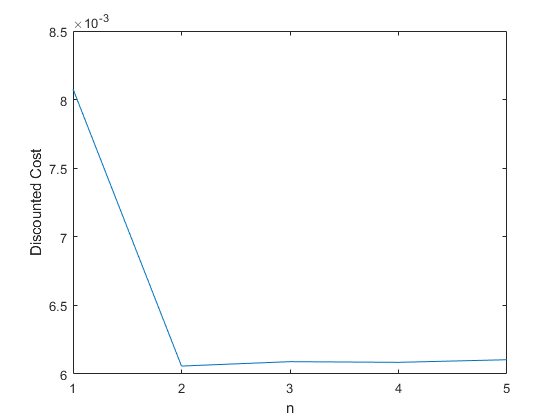
\includegraphics[height=6cm, width=10cm]{Cost_5.png}
    \caption{Long-term discounted cost of learned policies}
\end{figure}

\begin{figure}[H]
    \centering
    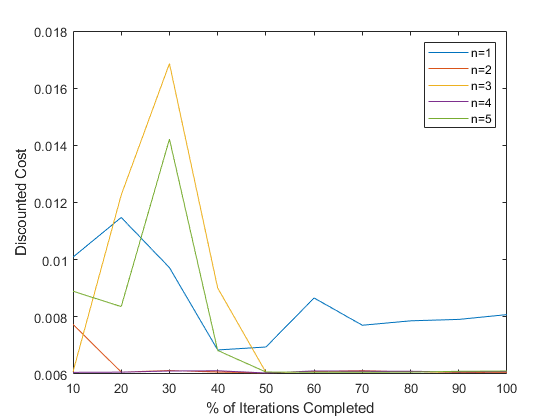
\includegraphics[height=6cm, width=10cm]{Quantization_5.png}
    \caption{Convergece of learned policies}
\end{figure}

Note that the quantization gains aren't significant after \( n=2 \) (which corresponds to 15 bins), which indicates that this is a sufficient quantization level for a near-optimal policy.

Similarly, we have the following graphs for \( \mathbb{X} = \{1,\ldots,16\} \).

\begin{figure}[H]
    \centering
    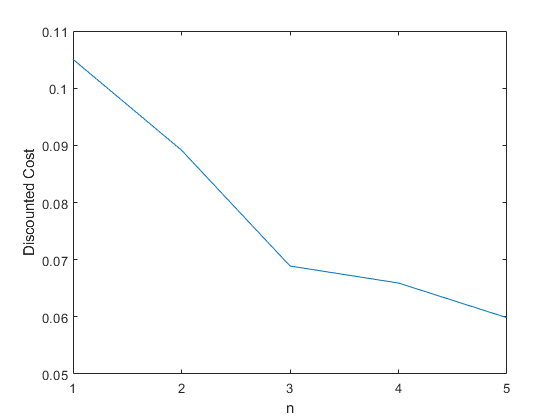
\includegraphics[height=6cm, width=10cm]{Cost_16.png}
    \caption{Long-term discounted cost of learned policies}
\end{figure}

\begin{figure}[H]
    \centering
    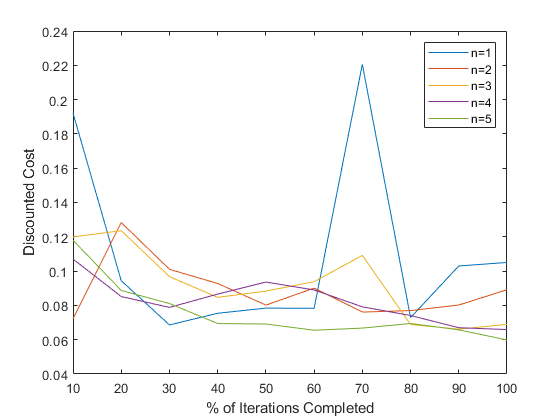
\includegraphics[height=6cm, width=10cm]{Quantization_16.png}
    \caption{Convergece of learned policies}
\end{figure}

Here, additional quantization may be required to get closer to the optimal policy. Unfortunately, the number of bins grows quickly with \(n\), and so further increasing the granularity becomes very computationally demanding. However, the number of actual visited states tends to be much lower than the total number of bins, and so it may be possible to increase the efficiency of this algorithm by restricting the state space of \(\pi_t\).

\section{Future Work}
We note that the above Q-learning algorithm only converges when \( \beta \in (0,1) \) (i.e.\ for the discounted cost problem) and therefore is not applicable for the average cost problem, which is generally what we are interested in for source coding. It may be possible to adapt the Q-learning algorithm to solve the average cost problem (see e.g.\ \cite{Abounadi}), but this would require an extension of the results in~\cite{Kara} to this algorithm, which may require additional constraints on the source \( \mathbb{X} \).

Furthermore, we would like to extend the algorithm to the case when \( \mathbb{X} \) is continuous. The primary obstable here would be that the number of possible quantizers is infinite, and so a method of quantizing the space of quantizers would need to be developed. We note however that quantizing the action space (in this context, the set of quantizers) is considered in the results from~\cite{Kara}, so convergence should follow with some minor alterations.

\printbibliography %chktex 1
\end{document} %chktex 17